%----------------------------------------------------------------------------------------
%	PACKAGES ET CONFIGURATION DU DOCUMENT
%----------------------------------------------------------------------------------------
\documentclass{article}

\usepackage[utf8]{inputenc} % Nécessaire pour les caractères internationaux
\usepackage[T1]{fontenc} % Encodage de polices pour les caractères internationaux
\usepackage{geometry}
\usepackage{graphicx}
\usepackage[french]{babel}
\usepackage{color, colortbl}
\usepackage{xcolor}
\usepackage{enumitem}
\usepackage{longtable}
\PassOptionsToPackage{hyphens}{url}\usepackage{hyperref}

\definecolor{Gray}{gray}{0.6}
\definecolor{Red}{HTML}{FF0000}
\definecolor{Green}{HTML}{00FF00}
\definecolor{Yellow}{HTML}{FFFF00}
\geometry{bottom=20 mm, top=20 mm}
%----------------------------------------------------------------------------------------

\begin{document}
\begin{titlepage}
	\centering
	
	{\huge Toi Plus} \\
    Nicolas Marier,
    Guillaume Rousseau,
    Thomas Garneau-Hamel,
    Charles-Antoine Demetriade \\
    420-204-RE, gr.1
    
    \vspace{6 cm}
    
    \huge{Dossier de conception} \\
    \large{Silence radio}
    
    \vspace{4 cm}
    
    Travail présenté à \\
    M. Walid Boulabiar
    
    \vspace{8 cm}
    
    Département d'informatique \\
    Cégep Limoilou \\
    Le 6 février 2019
\end{titlepage}
\tableofcontents

\newpage

\section{Description du projet}
    \paragraph{Objectifs :}
Le besoin auquel notre projet vise à répondre est la transmission de données sans fil.
Pour répondre au besoin, il faut que la transmission soit sécuritaire et privée.
De plus, il faut être en mesure de détecter et corriger les erreurs de transmission d'information, afin d'éviter la corruption de l'information.
Notre projet répond également au besoin grandissant de comprendre en détail le fonctionnement d'Internet et les principes fondamentaux physiques et mathématiques qui permettent l'utilisation d'un tel réseau.

\paragraph{Description détaillée :}
Au plus haut niveau, l'application sera utilisée de la façon suivante : l'utilisateur commence par sélectionner un fichier de son choix, de n'importe quel type et de n'importe quel format, qu'il veut envoyer à un autre ordinateur. Ensuite, le logiciel se charge de convertir le fichier de l'utilisateur dans un format binaire sérialisé. Le fichier, sous forme binaire, est converti à nouveau sous un format analogue qui sera un son pour émettre du courant alternatif dans notre circuit. Le son sera sélectionné très précisément, car il est responsable de la modulation de la fréquence de notre once ainsi que de l'amplitude de celle-ci. L'utilisation du son à cet effet permettra à l'utilisateur de choisir lui-même la fréquence sur laquelle il désire transmettre l'information. Le son sera transformé en onde électromagnétique par notre circuit RLC et reçu par notre autre circuit de réception. Une fois reçu par le récepteur, connecté à un second ordinateur, les ondes électromagnétiques seront reconverties en binaire, pour ultimement recréer l'information d'origine. S'il advenait qu'une erreur de transmission se produise, elle serait corrigée, si notre système de correction d'erreurs le permet. Sinon, l'ordinateur receveur avertira l'utilisateur de la corruption de son information et l'invitera à réinitialiser le transfert

\paragraph{Concepts :}
\begin{itemize}
    \item Circuits électriques
    \begin{itemize}
        \item Calculs pour déterminer les composantes
        \item Circuits RLC
        \item Courant alternatif
    \end{itemize}
    \item Ondes électromagnétiques
    \begin{itemize}
        \item Fréquence 
        \item Amplitude
        \item Ondes AM 
    \end{itemize}
    \item Correction et détection d'erreurs
    \item Sérialisation d'objets en blob (\textbf{b}inary \textbf{l}arge \textbf{ob}ject)
    \item Conversion digital to analog et analog to digital
    \item Interprétation du flux binaire reçu pour reconstruire l'information
\end{itemize}

\paragraph{Nouveaux concepts :}
Tout ce qui a trait aux ondes est nouveau pour nous étant donné que nous sommes en train de compléter le cours d'ondes et physique moderne.
Malgré le fait que nous avons fait des circuits dans le cours de physique précédent, ils étaient théoriques.
Nous n'avons que très rarement assemblé des circuits, et nous ne les avons jamais élaborés nous-mêmes.
La conversion digital to analog nécessaire à l'envoi d'ondes est quelque chose que nous n'avons jamais fait.
Aussi, nous n'avons jamais transmis d'ondes entre deux circuits.
Il nous faudra également apprendre les principes de correction d'erreurs pour détecter et corriger les erreurs.

\paragraph{Complexité :}
La complexité provient surtout du fait que nous avons beaucoup de choses à apprendre.
Il est difficile d'évaluer correctement la complexité du projet étant donné notre inexpérience dans les nouveaux concepts.
Cependant, nous pouvons dire avec certitude que la tâche ne sera pas si facile, car la contrainte de temps est concidérable.
De plus, les nombreuses tâches du projet vont nécessiter une attention particulière, étant donné que le succès de chaque étape est obligatoire pour l'élaboration de l'étape suivante.
Nous sommes convaincus de la possibilité de réaliser le projet, car il est possible de retirer certains facteurs de complexité s'il s'avère que notre entreprise était initialement trop ambitieuse.
Notre professeur de physique nous a confirmé qu'il allait pouvoir nous aider en cas de besoin, et qu'il est certain que la réalisation du projet est possible.

\paragraph{Concepts, rôles et justifications : }
\begin{itemize}
    \item Nicolas Marier, chef et développeur
    \item Thomas Garneau-Hamel, électronique, physicien et motivateur
    \item Guillaume Rousseau, documentation et physicien
    \item Charles-Antoine Demetriade, graphiques/interfaces
\end{itemize}
Nous avons choisi ces rôles en fonction de nos forces et nos goûts ainsi que nos faiblesses.

\paragraph{Séparation des tâches :}
\begin{itemize}
    \item Nicolas Marier : élaboration de la programmation des classes métier ainsi que des diagrammes UML.
    \item Thomas Garneau-Hamel : conception du circuit électrique et calculs.
    \item Guillaume Rousseau : documentation, recherche, contrôle de qualité.
    \item Charles-Antoine Demetriade : création de la vue et de ce qui se rapporte à l'environnement graphique.
\end{itemize}

\paragraph{Type d'application :}
Windows, Mac, Linux (exécutable par la JVM)
\paragraph{Languages utilisés, patrons de conception :}
\begin{itemize}
    \item Language : Java
    \item Patrons de conception : MVC
\end{itemize}

\paragraph{Technologies impliquées :}
\begin{itemize}
    \item IDE: Eclipse, IntelliJ, SceneBuilder, PlantUML
    \item Hardware : un ordinateur et un raspberry pi, des composantes élctroniques (résistances, condensateurs, fils)
\end{itemize}

\paragraph{Références et documentation :}
\begin{itemize}
    \item \url{https://electronics.howstuffworks.com/radio.htm}
    \item \url{http://www.ta-formation.com/acrobat/am.pdf}
    \item \url{http://ekladata.com/I91iUA5sMDI3QLRiLD82FmviNF4/TX-AM.pdf}
    \item \url{http://www.cea.fr/comprendre/Pages/physique-chimie/essentiel-sur-ondes-electromagnetiques-communication.aspx}
\end{itemize}

\section{Prototypes de l'application}
    \paragraph{Prototype :}
Nous aimerions que notre interface ait un thème de cockpit d'avion.
Donc, les couleurs choisies ainsi que la police de caractère que nous sélectionnerons reflèteront cette esthétique.
\begin{figure}[ht!]
    \centering
    \caption{Prototype de l'interface}
    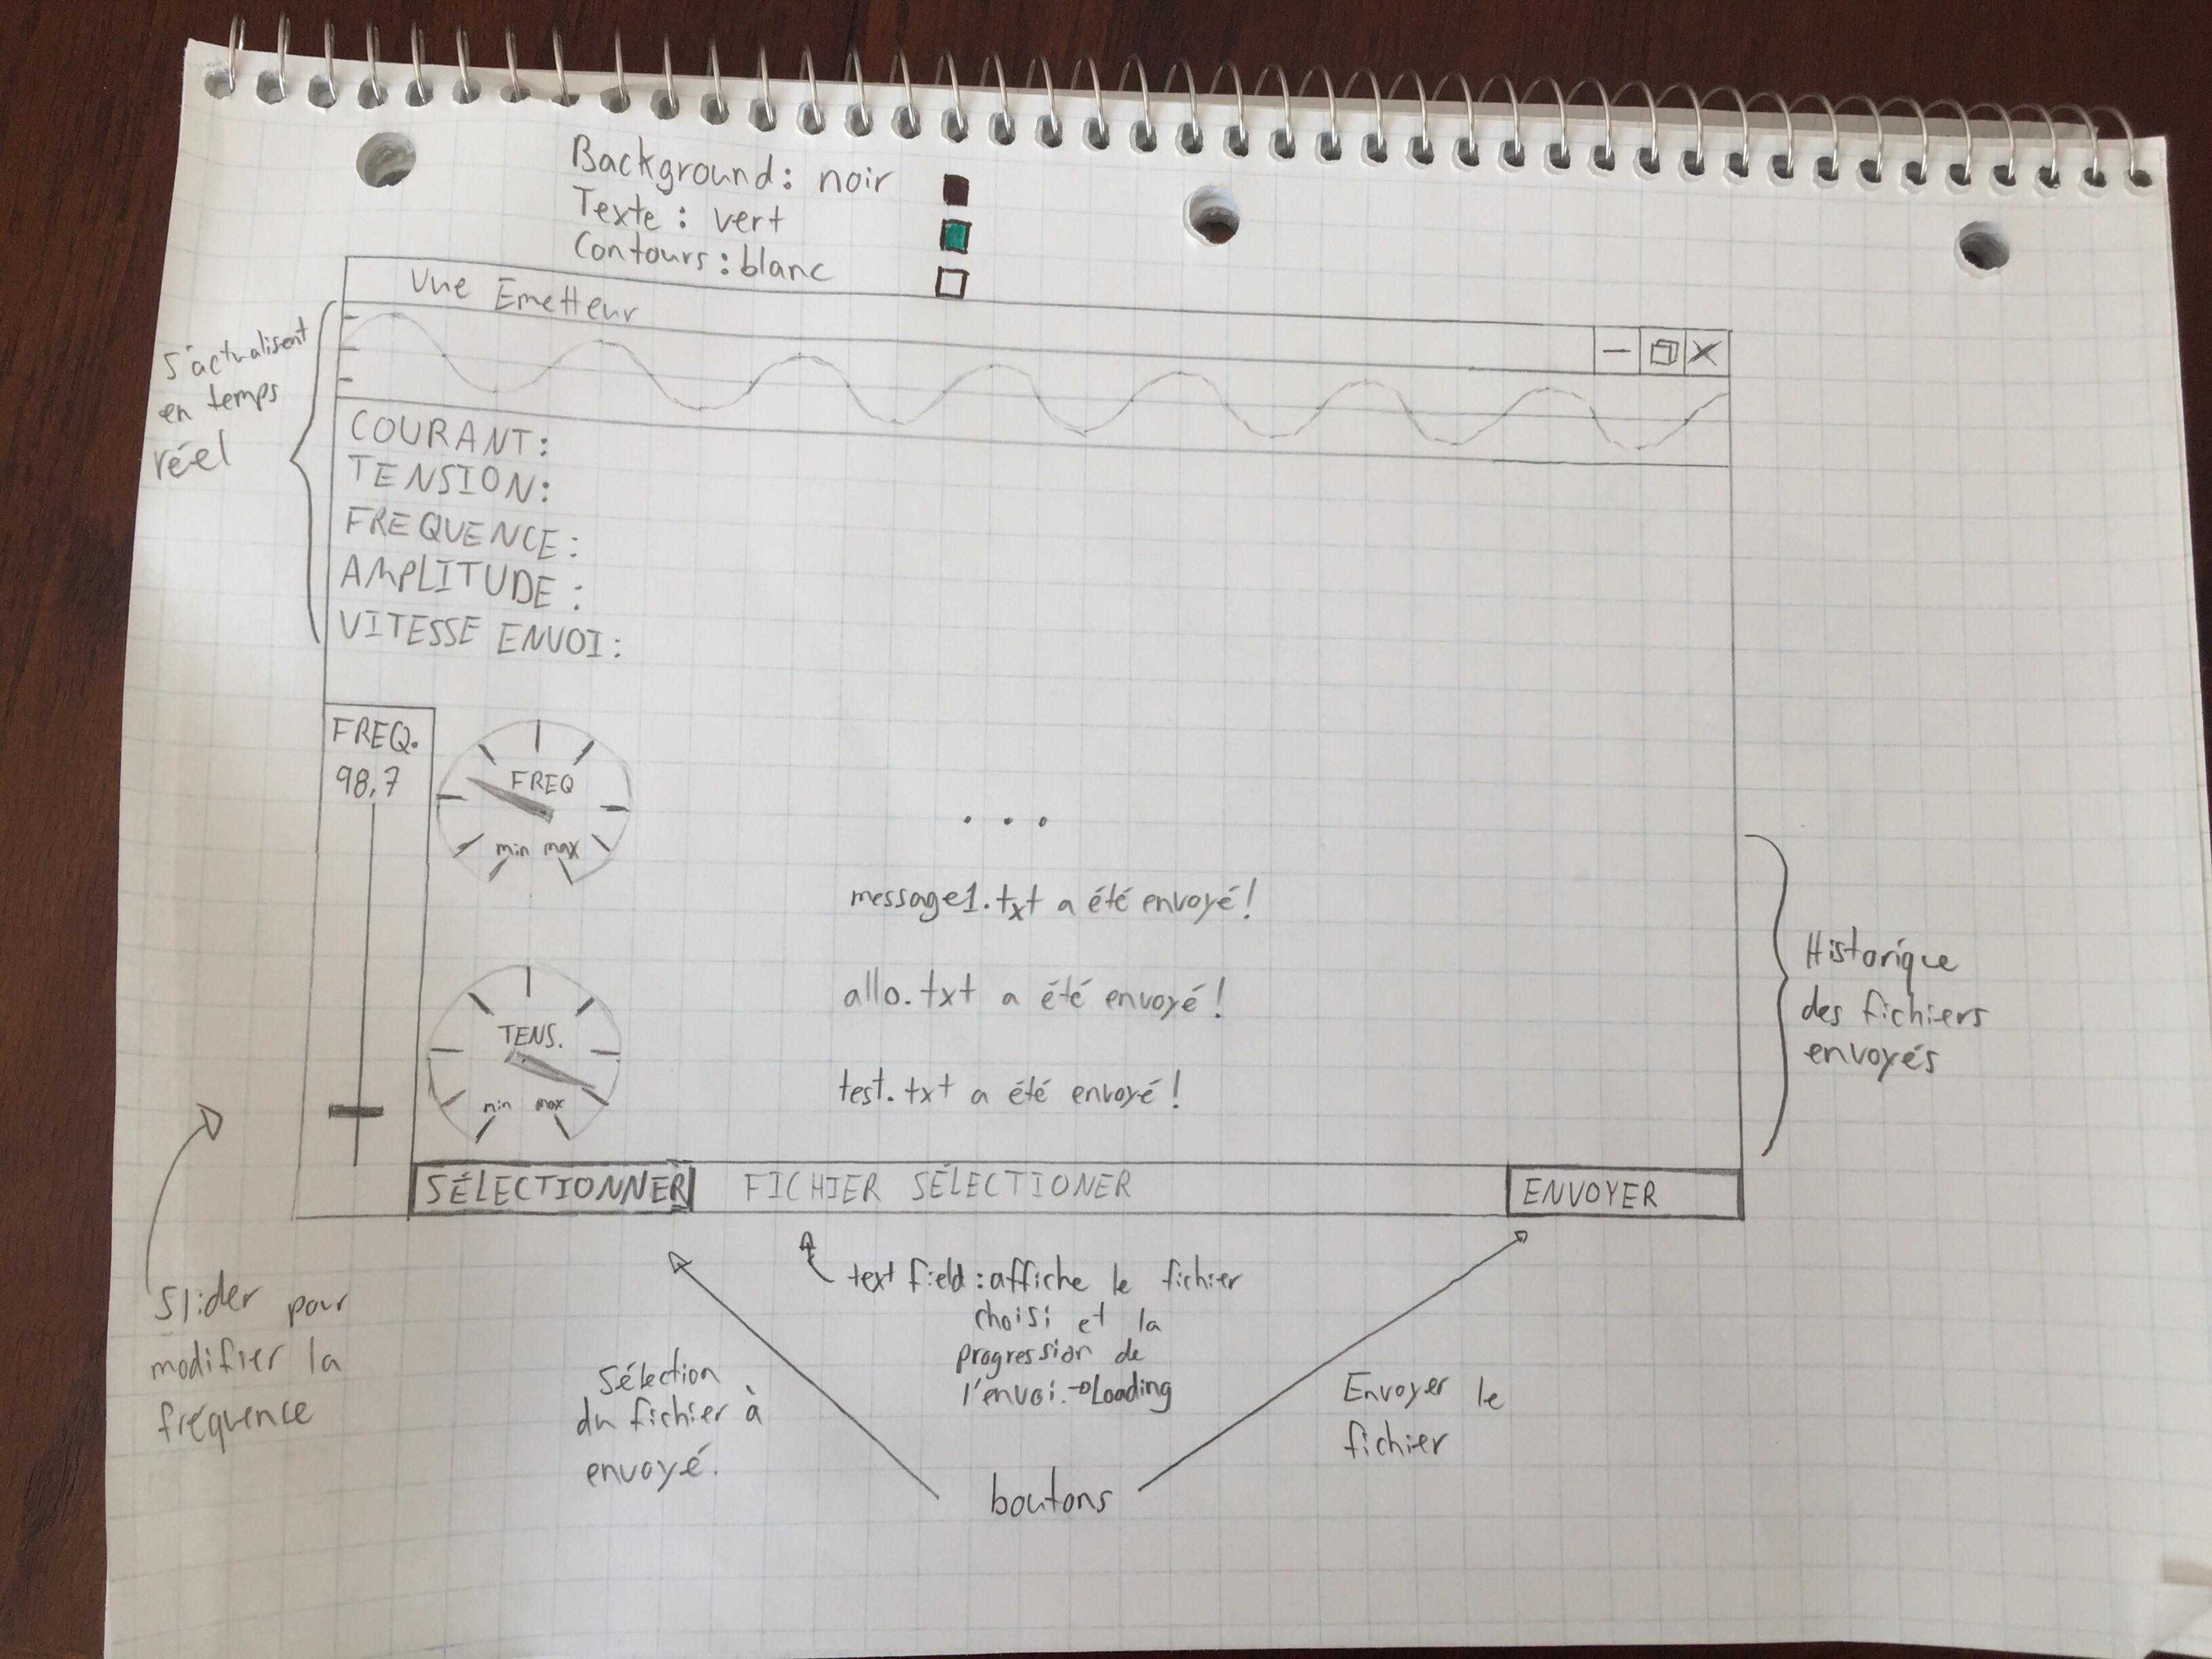
\includegraphics[width=0.8\linewidth]{images/proto/interface_graphique.jpg}
\end{figure}

\newpage

\paragraph{Principaux objets :} 
\begin{itemize}
    \item Visualisation des ondes envoyées
    \item Valeurs pour les différents paramètres 
    \begin{itemize}
        \item Courant dans le circuit
        \item Tension sur le circuit
        \item Fréquence sur laquelle on émet
        \item Amplitude des ondes
        \item Vitesse d'envoi (B/sec ou KB/sec)
    \end{itemize}
    \item La liste des fichiers envoyés
    \item Des boutons pour choisir un fichier et l'envoyer
    \item Un contrôle pour modifier la fréquence
    \item Des visualisations pour la fréquence et la tension relative (pour savoir si on s'approche du maximum permis)
    \item Potentiellement à ajouter serait un indicateur de puissance utilisée par le circuit
\end{itemize}

\begin{figure}[ht!]
    \centering
    \caption{Prototype du physique}
    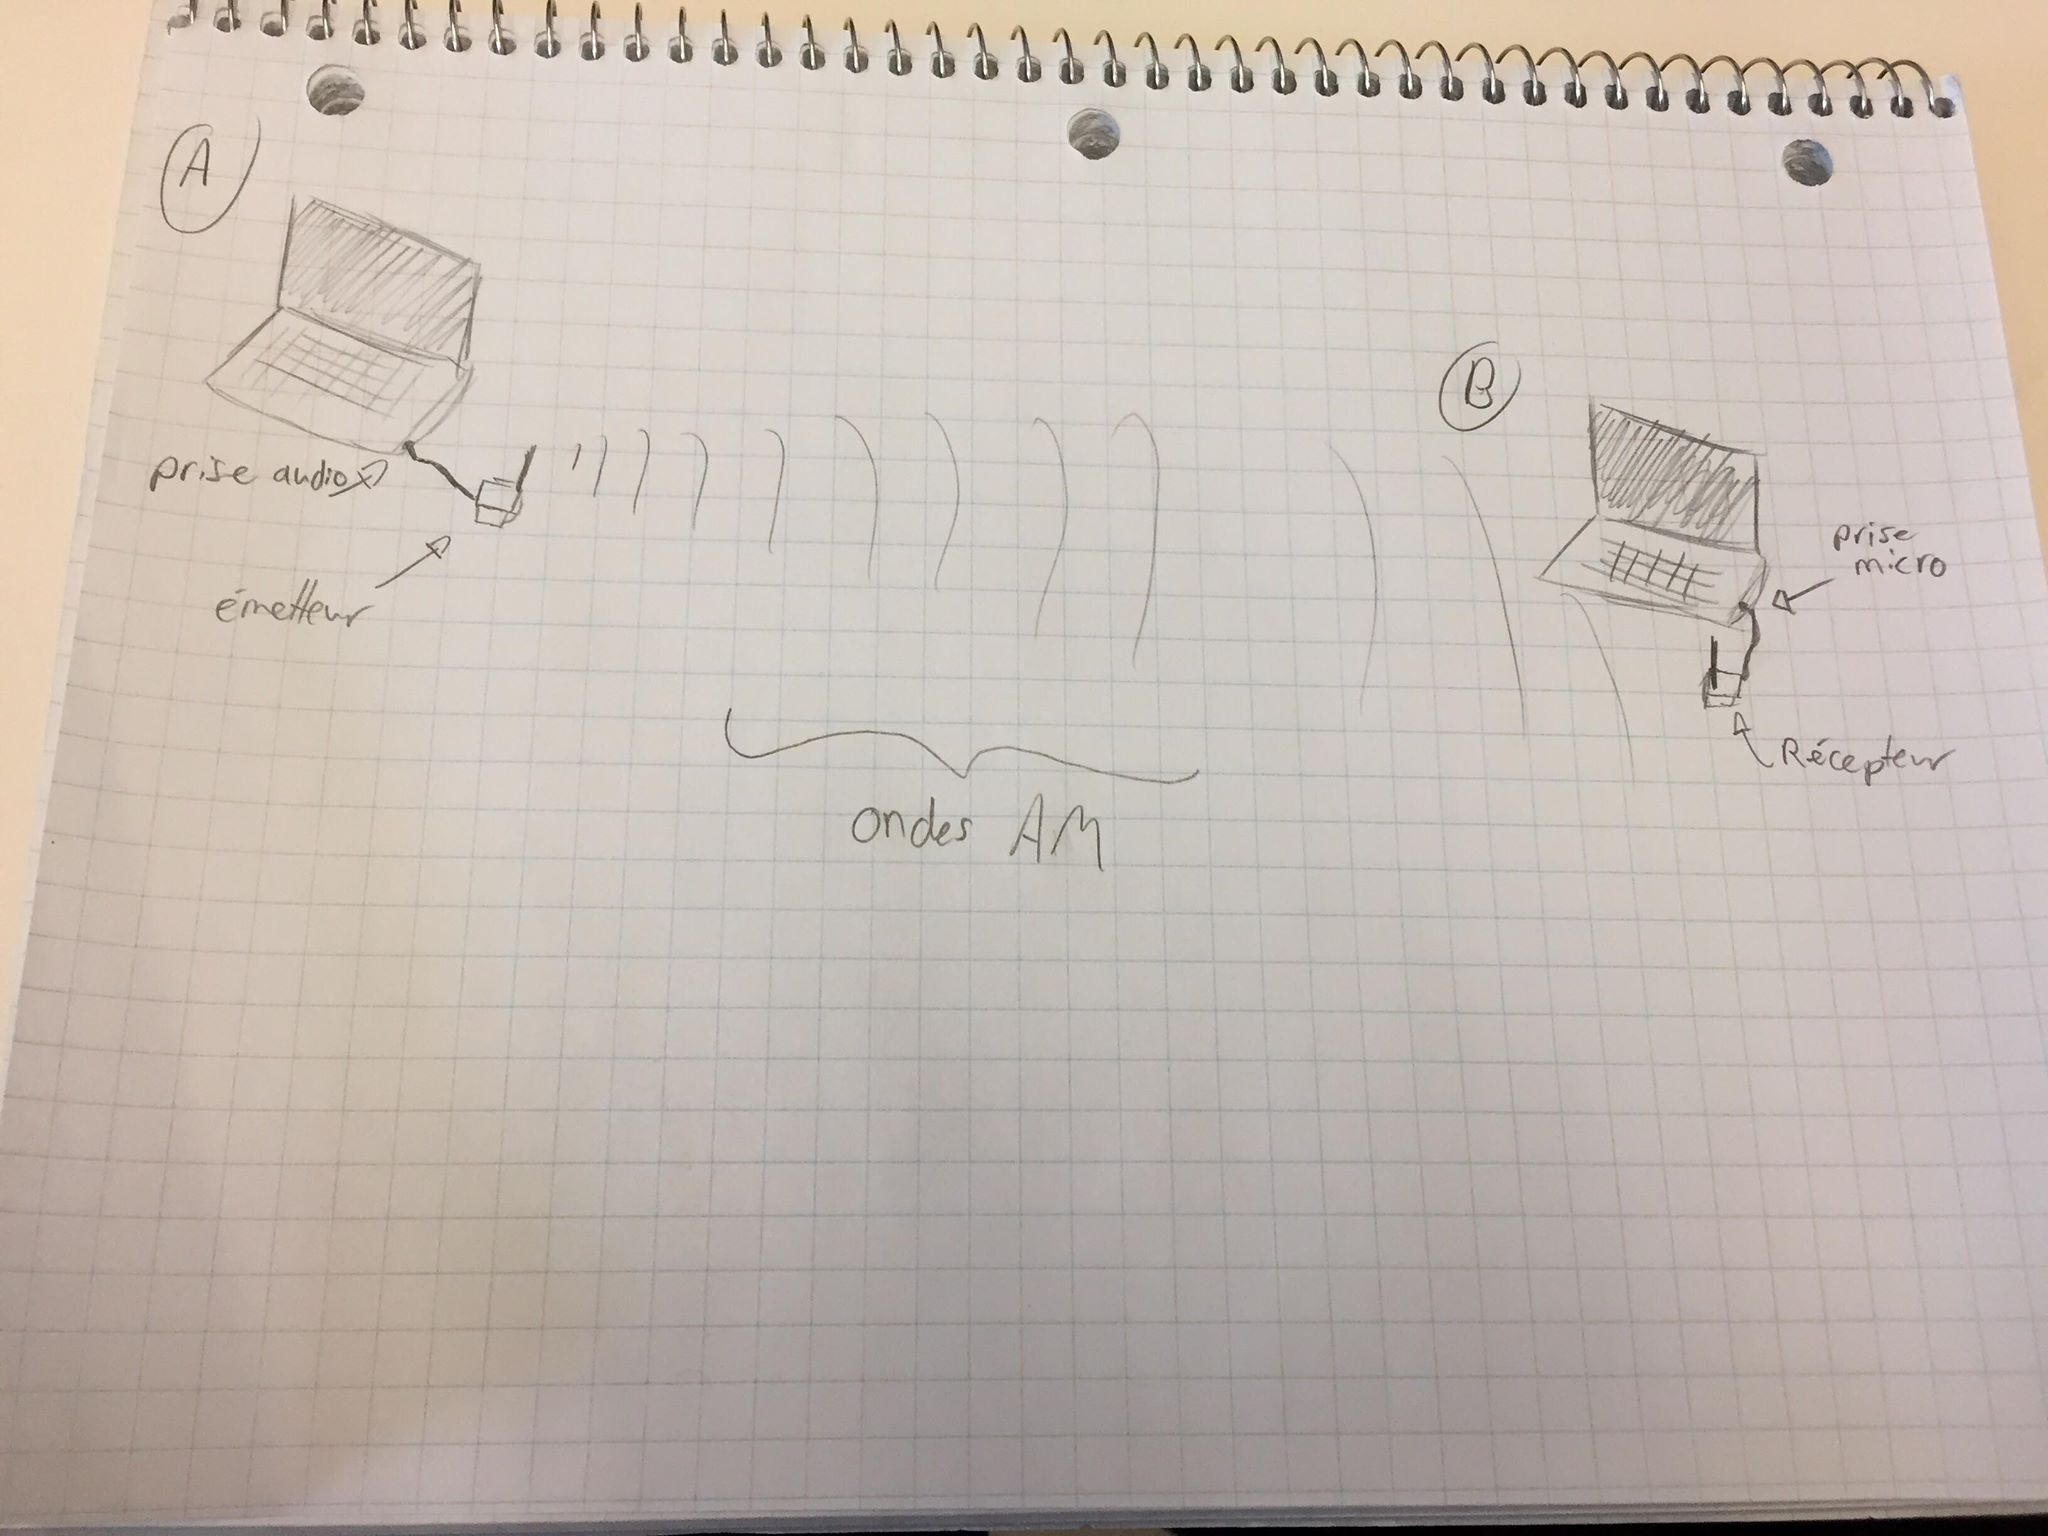
\includegraphics[width=0.4\linewidth]{images/proto/visualisation_transmission.jpg}
\end{figure}

\newpage

\newgeometry{left=15mm, right=15mm, bottom=20mm, top=20mm}
\section{Backlogs}
    \subsection{Backlog de produit}
        \begin{longtable}{|l|p{0.8\textwidth}|}
\multicolumn{2}{r}{Suite à la page suivante} \\
\endfoot

\multicolumn{2}{r}{} \\
\endlastfoot

\hline
    \rowcolor{Gray}
    \multicolumn{2}{|l|}{1} \\
\hline
    Acteur ou rôle & Utilisateur \\
\hline
    Scénario ou story & \colorbox{Green}{\parbox{14.5cm}{En tant qu'utilisateur, 
      je veux pouvoir sélectionner un fichier
      afin de pouvoir l'envoyer.}} \\
\hline
    Détail et description & 
    Avoir accès à son explorateur de fichier dans le but de pouvoir sélectionner n'importe lequel fichier disponible dans les archives \\
       
\hline
    Tests d'acceptation & Sélectionner un fichier et vérifier qu'il s'affiche correctement. \\
\hline
    Complexité & 1 \\
\hline
    Effort & 1 \\
\hline
    Commentaires &  \\

\hline
    \rowcolor{Gray}
    \multicolumn{2}{|l|}{2} \\
\hline
    Acteur ou rôle & Utilisateur \\
\hline
    Scénario ou story & En tant qu'utilisateur,
          je souhaite que le logiciel soit capable de détecter
          si le transfert de fichiers s'est bien complété et que
          ce dernier puisse corriger l'information reçue si cette
          dernière comprend des erreurs.\\
\hline
    Détail et description & En cas de corruption lors du transfert de données, le logiciel détecte l'emplacement du problème et offre à l'utilisateur de corriger les erreurs rencontrées afin d'avoir des données complètes.\\
\hline
    Tests d'acceptation & Des bits de confirmation seront ajoutés à l'information. Il y aura un système de vérification inspiré du International Standard Book Number\\
\hline
    Complexité & 1 \\
\hline
    Effort & 1 \\
\hline
    Commentaires &  \\

\hline
    \rowcolor{Gray}
    \multicolumn{2}{|l|}{3} \\
\hline
    Acteur ou rôle & Programmeur\\
\hline
    Scénario ou story &  \colorbox{Green}{\parbox{14.5cm}{En tant que programmeur,
          je dois pouvoir convertir l'information contenue 
          dans le fichier sélectionné en code binaire afin que ces 
          dernières soient plus faciles à transmettre par ondes radio.}} \\
\hline
    Détail et description & Pouvoir prendre n'importe quel type de fichier et le convertir en binaire, soit en suite de 1 et de 0, dans le but de faciliter la transmission par ondes radio puisque le binaire est beaucoup plus simple à représenter par des ondes.
        \\
\hline
    Tests d'acceptation & Comparaison de la conversion en binaire avec un fragment du fichier connu. \\

\hline
    Complexité & 1 \\
\hline
    Effort & 2 \\
\hline
    Commentaires &  \\

\hline
    \rowcolor{Gray}
    \multicolumn{2}{|l|}{4} \\
\hline
    Acteur ou rôle & Développeur \\
\hline
    Scénario ou story & En tant que développeur,
          je veux que le code binaire soit converti en son afin de permettre à l'information d'être envoyée par l'antenne de transmission. \\
\hline
    Détail et description & Avec le son nouvellement transformé, il sera alors possible de créer un courant alternatif qui permettra par la suite de créer plus facilement des ondes. \\
\hline
    Tests d'acceptation & Tests sonores ainsi que des tests à l'aide d'un multimètre. \\
\hline
    Complexité & 2 \\
\hline
    Effort & 3 \\
\hline
    Commentaires &  \\

\hline
    \rowcolor{Gray}
    \multicolumn{2}{|l|}{5} \\
\hline
    Acteur ou rôle & Physicien \\
\hline
    Scénario ou story &  \colorbox{Green}{\parbox{14.5cm}{En tant que physicien,
          je veux posséder un circuit émetteur afin de pouvoir envoyer les ondes radio contenant l'information du fichier sélectionné.}}\\
\hline
    Détail et description & Un circuit électrique de courant alternatif composé de résistance, de condensateurs et de bobines inductives. \\
\hline
    Tests d'acceptation & Tests techniques avec un multimètre et des tests pour les ondes avec une radio \\
\hline
    Complexité & 3 \\
\hline
    Effort & 6 \\
\hline
    Commentaires &  \\

\hline
    \rowcolor{Gray}
    \multicolumn{2}{|l|}{6} \\
\hline
    Acteur ou rôle & Utilisateur \\
\hline
    Scénario ou story & En tant qu'utilisateur,
          je veux posséder un circuit récepteur afin de pouvoir capter les ondes radio produites par l'émetteur. \\
\hline
    Détail et description & Un circuit électrique de courant alternatif composé de résistance, de condensateurs et de bobines inductives. \\
\hline
    Tests d'acceptation & Tests techniques avec un multimètre \\
\hline
    Complexité & 3 \\
\hline
    Effort & 6 \\
\hline
    Commentaires &  \\

\hline
    \rowcolor{Gray}
    \multicolumn{2}{|l|}{7} \\
\hline
    Acteur ou rôle & Développeur \\
\hline
    Scénario ou story &  En tant que développeur,
          les courants électriques créés par la réception d'ondes radio doivent 
          m'être convertis en binaire afin que ces derniers puissent être interprétés 
          par l'ordinateur. \\
\hline
    Détail et description & Selon les caractéristiques des ondes reçues, les reconvertir en binaire. \\
\hline
    Tests d'acceptation & Test de conversion avec des valeurs connues prédéterminées \\
\hline
    Complexité & 3 \\
\hline
    Effort & 4 \\
\hline
    Commentaires &  \\

\hline
    \rowcolor{Gray}
    \multicolumn{2}{|l|}{8} \\
\hline
    Acteur ou rôle & Programmeur \\
\hline
    Scénario ou story & En tant que programmeur,
          je dois être en mesure de reconstruire le fichier envoyé par l'émetteur à partir du code binaire reçu. \\
\hline
    Détail et description & Effectuer la reconstruction du fichier d'origine en utilisant seulement ce qui a été reçu par l'antenne de réception \\
\hline
    Tests d'acceptation & Tests avec des fichiers connus\\
\hline
    Complexité & 1 \\
\hline
    Effort & 1 \\
\hline
    Commentaires &  \\

\hline
    \rowcolor{Gray}
    \multicolumn{2}{|l|}{9} \\
\hline
    Acteur ou rôle & Utilisateur \\
\hline
    Scénario ou story &  En tant qu'utilisateur,
          je souhaite pouvoir avoir une représentation visuelle
          du progrès du transfert des fichiers afin de me permettre
          de savoir quand ce dernier est fini et afin d'ajouter un
          élément esthétique à l'interface. \\
\hline
    Détail et description & Avoir accès visuellement à la progression de l'envoi du fichier à l'aide d'une barre de progrès \\
\hline
    Tests d'acceptation & Tests avec des fichiers de grosseur connues\\
\hline
    Complexité & 1 \\
\hline
    Effort & 2 \\
\hline
    Commentaires &  \\

\hline
    \rowcolor{Gray}
    \multicolumn{2}{|l|}{10} \\
\hline
    Acteur ou rôle & Utilisateur \\
\hline
    Scénario ou story &  En tant qu'utilisateur,
          je dois pouvoir sélectionner la fréquence radio sur laquelle je
          souhaite faire mon transfert d'information afin de pouvoir choisir celle 
          qui possède le moins d'interférences pouvant affecter négativement le transfert d'informations. \\
\hline
    Détail et description & Être en mesure de choisir la fréquence désirée, celle avec le moins d'interférence, dans le but d'assurer un meilleur transfert de données \\
\hline
    Tests d'acceptation & Tests avec une radio\\
\hline
    Complexité & 1 \\
\hline
    Effort & 1 \\
\hline
    Commentaires &  \\

\hline
    \rowcolor{Gray}
    \multicolumn{2}{|l|}{11} \\
\hline
    Acteur ou rôle & Utilisateur \\
\hline
    Scénario ou story & \colorbox{Green}{\parbox{14.5cm}{En tant qu'utilisateur,
          je dois avoir une interface visuelle de l'émetteur afin
          de pouvoir visualiser et sélectionner le fichier.}}\\
\hline
    Détail et description & Interface graphique suivant la thématique d'un cockpit, c'est-à-dire une interface comportant toutes les données du circuit et du transfert de données qui sont importantes. \\
\hline
    Tests d'acceptation & Tests visuels\\
\hline
    Complexité & 2 \\
\hline
    Effort & 3\\
\hline
    Commentaires &  \\

\hline
    \rowcolor{Gray}
    \multicolumn{2}{|l|}{12} \\
\hline
    Acteur ou rôle & Utilisateur \\
\hline
    Scénario ou story & En tant qu'utilisateur,
          je dois avoir une interface dédiée à la réception des
          fichiers en transfert afin de pouvoir mieux gérer
          l'enregistrement de ces derniers.\\
\hline
    Détail et description & Interface comportant l'historique des réceptions de fichiers ainsi qu'un moyen intuitif pour enregistrer ce qui a été reçu.\\
\hline
    Tests d'acceptation & Tests visuels\\
\hline
    Complexité & 1 \\
\hline
    Effort & 2\\
\hline
    Commentaires &  \\

\hline
    \rowcolor{Gray}
    \multicolumn{2}{|l|}{13} \\
\hline
    Acteur ou rôle & Utilisateur \\
\hline
    Scénario ou story & En tant qu'utilisateur,
          je dois être en mesure de sélectionner où est enregistré
          le fichier que je reçois afin d'éviter de le perdre ou
          qu'il ne s'enregistre nulle part.\\
\hline
    Détail et description & Avoir accès à l'explorateur de fichier dans le but de pouvoir enregistrer de manière simple et efficace.\\
\hline
    Tests d'acceptation & Tests unitaires\\
\hline
    Complexité & 1 \\
\hline
    Effort & 1\\
\hline
    Commentaires &  \\

\hline
    \rowcolor{Gray}
    \multicolumn{2}{|l|}{14} \\
\hline
    Acteur ou rôle & Administrateur \\
\hline
    Scénario ou story & En tant qu'administrateur,
          je souhaite que la fréquence radio de l'émetteur se choisisse automatiquement
          afin qu'elle choisisse elle-même la meilleure fréquence radio pour faire le transfert.\\
\hline
    Détail et description & Le logiciel de l'émetteur soit en mesure de trouver la meilleure fréquence par lui-même afin de choisir automatique cette fréquence dans le but d'effectuer le meilleur transfert de données possibles.\\
\hline
    Tests d'acceptation & Tests pratiques et comparaison avec la fréquence connue\\
\hline
    Complexité & 3 \\
\hline
    Effort & 6\\
\hline
    Commentaires &  \\

\hline
    \rowcolor{Gray}
    \multicolumn{2}{|l|}{15} \\
\hline
    Acteur ou rôle & Utilisateur \\
\hline
    Scénario ou story &  En tant qu'utilisateur,
          je dois être en mesure de décider laquelle des interfaces visuelles je souhaite
          utiliser afin de me permettre d'utiliser le logiciel adéquatement.\\
\hline
    Détail et description & En démarrant l'application, il y a l'option de sélectionner le mode émetteur ou bien le mode de récepteur. \\
\hline
    Tests d'acceptation & Tests visuels\\
\hline
    Complexité & 1 \\
\hline
    Effort & 1\\
\hline
    Commentaires &  \\

\hline
    \rowcolor{Gray}
    \multicolumn{2}{|l|}{16} \\
\hline
    Acteur ou rôle & Administrateur \\
\hline
    Scénario ou story &  En tant qu'administrateur, je souhaite sécuriser la
          communication afin de rendre celle-ci privée.\\
\hline
    Détail et description & Rendre la communication plus sécurisée en cryptant les données à envoyer afin d'éviter les vols d'informations \\
\hline
    Tests d'acceptation & Tests visuels\\
\hline
    Complexité & 4 \\
\hline
    Effort & 8\\
\hline
    Commentaires &  \\
\hline
\end{longtable}




\newpage

    \subsection{Backlog de sprint \#1}
        \begin{longtable}{|l|p{0.8\textwidth}|}
\multicolumn{2}{r}{Suite à la page suivante} \\
\endfoot

\multicolumn{2}{r}{} \\
\endlastfoot

\hline
    \rowcolor{Gray}
    \multicolumn{2}{|l|}{1} \\
\hline
    Acteur ou rôle & Utilisateur \\
\hline
    Scénario ou story & En tant qu'utilisateur, 
      je veux pouvoir sélectionner un fichier
      afin de pouvoir l'envoyer. \\
\hline
    Détail et description &
        \begin{enumerate}[label*=\arabic*.]
            \item \colorbox{Green}{\parbox{13cm}{Permettre à l’utilisateur d’accéder à sa bibliothèque de fichiers.}}
            \begin{enumerate}[label*=\arabic*.]
                    \item Qui et temps :
                    \begin{enumerate}[label*=\arabic*.]
                        \item (NM)
                        \item (30 minutes)
                    \end{enumerate}
                    \item Préconditions : 
                    \begin{enumerate}[label*=\arabic*.]
                        \item La présence d'un bouton qui permet à l'utilisateur de procéder à l'action de sélectionner un fichier.
                    \end{enumerate}
                    \item Règles d’affaires :
                    \begin{enumerate}[label*=\arabic*.]
                        \item Doit sélectionner un fichier existant dans l'espace de donné de l'ordinateur utilisé.
                    \end{enumerate}
                    \item Règles d’affaires alternatives :
                    \begin{enumerate}[label*=\arabic*.]
                        \item S'il ne sélectionne pas un fichier existant ou que le fichier sélectionné n'existe plus une fois sélectionné, une alerte est envoyé à l'utilisateur afin qu'il en sélectionne un nouveau.
                    \end{enumerate}
                    \item Tests d'acceptation de cet item :
                    \begin{enumerate}[label*=\arabic*.]
                        \item Tester si le fichier sélectionné est existant dans la base de donnée de l'ordinateur et accessible par le logiciel.
                        \item Vérifier que le contenu du fichier est lisible par le logiciel.
                    \end{enumerate}
                    \item Post-conditions :
                    \begin{enumerate}[label*=\arabic*.]
                        \item L'utilisateur peut sélectionner le fichier qu'il souhaite émettre.
                    \end{enumerate}
                \end{enumerate}
            \item \colorbox{Green}{\parbox{13cm}{Présenter à l’utilisateur les informations du fichier qu’il s’apprête à envoyer.}}
                \begin{enumerate}[label*=\arabic*.]
                    \item Qui et temps :
                    \begin{enumerate}[label*=\arabic*.]
                        \item (NM)
                        \item (30 minutes)
                    \end{enumerate}
                    \item Préconditions : 
                    \begin{enumerate}[label*=\arabic*.]
                        \item Le fichier doit être sélectionné.
                    \end{enumerate}
                    \item Règles d’affaires :
                    \begin{enumerate}[label*=\arabic*.]
                        \item Doit pouvoir envoyer l'information à la vue du nom du fichier.
                    \end{enumerate}
                    \item Règles d’affaires alternatives :
                    \begin{enumerate}[label*=\arabic*.]
                        \item Si le nom comportes des caractères non interprétables par l'ordinateur, ce dernier ne les affichera pas.
                    \end{enumerate}
                    \item Tests d'acceptation de cet item :
                    \begin{enumerate}[label*=\arabic*.]
                        \item vérifier chacun des caractère du nom d'un fichier afin de pouvoir afficher tous ceux possibles.
                    \end{enumerate}
                    \item Post-conditions :
                    \begin{enumerate}[label*=\arabic*.]
                        \item L'utilisateur peut voir le nom de son fichier.
                    \end{enumerate}
                \end{enumerate}
        \end{enumerate} \\
\hline
    Tests d'acceptation & Sélectionner un fichier et vérifier qu'il s'affiche correctement. \\
\hline
    Complexité & 1 \\
\hline
    Effort & 1 \\
\hline
    Commentaires &  \\

\hline
    \rowcolor{Gray}
    \multicolumn{2}{|l|}{2} \\
\hline
    Acteur ou rôle & Utilisateur \\
\hline
    Scénario ou story & En tant qu’utilisateur, je
    dois posséder une interface
    visuelle pour l’émission des
    fichiers. \\
\hline
    Détail et description &
        \begin{enumerate}[label*=\arabic*.]
            \item \colorbox{Green}{\parbox{13cm}{Construire une interface avec
                la disposition souhaitée et les
                fonctions de bases permettant
                d’envoyer un fichier.}}
                \begin{enumerate}[label*=\arabic*.]
                                \item Qui et temps :
                                \begin{enumerate}[label*=\arabic*.]
                                    \item (CAD)
                                    \item (2h)
                                \end{enumerate}
                                \item Préconditions :
                                \begin{enumerate}[label*=\arabic*.]
                                    \item Avoir préparer un croquis de l'interface.
                                    \item Avoir le logiciel Scene Builder pour la conception de l'interface.
                                \end{enumerate}
                                \item Règles d'affaires :
                                \begin{enumerate}[label*=\arabic*.]
                                    \item Afficher l'interface de l'émetteur.
                                \end{enumerate}
                                \item Règles d'affaires alternatives :
                                \begin{enumerate}[label*=\arabic*.]
                                    \item Il n'y a pas d'alternative, car sans interface, l'utilisateur ne peut rien faire.
                                \end{enumerate}
                                \item Tests d'acceptation de cet item :
                                \begin{enumerate}[label*=\arabic*.]
                                    \item Les tests seront au niveau visuel. S'il y a un problème d'affichage, on pourra le voir.
                                \end{enumerate}
                                \item Post-conditions :
                                \begin{enumerate}[label*=\arabic*.]
                                    \item L'interface devra pouvoir afficher les éléments suivant : Boutons pour la sélections, envoies de fichier.
                                \end{enumerate}
                            \end{enumerate}
             \item \colorbox{Green}{\parbox{13cm}{Ajouter à l’interface de la couleur et du style.}}
                \begin{enumerate}[label*=\arabic*.]
                                \item Qui et temps :
                                \begin{enumerate}[label*=\arabic*.]
                                    \item (CAD)
                                    \item (1h)
                                \end{enumerate}
                                \item Préconditions :
                                \begin{enumerate}[label*=\arabic*.]
                                    \item Avoir terminé le fxml.
                                \end{enumerate}
                                \item Règles d'affaires :
                                \begin{enumerate}[label*=\arabic*.]
                                    \item Styliser l'interface en css.
                                \end{enumerate}
                                \item Règles d'affaires alternatives :
                                \begin{enumerate}[label*=\arabic*.]
                                    \item Il n'y a pas d'alternative.
                                \end{enumerate}
                                \item Tests d'acceptation de cet item :
                                \begin{enumerate}[label*=\arabic*.]
                                    \item Les tests seront au niveau visuel. S'il y a un problème d'affichage, on pourra le voir.
                                \end{enumerate}
                                \item Post-conditions :
                                \begin{enumerate}[label*=\arabic*.]
                                    \item L'interface devra être en noir, vert et blanc comme une vue de console.
                                \end{enumerate}
                            \end{enumerate}                
        \end{enumerate} \\
\hline
    Tests d'acceptation & Les tests seront au niveau visuel. S'il y a un problème d'affichage, on pourra le voir. \\
\hline
    Complexité & 1 \\
\hline
    Effort & 1 \\
\hline
    Commentaires &  \\

\hline
    \rowcolor{Gray}
    \multicolumn{2}{|l|}{3} \\
\hline
    Acteur ou rôle & Utilisateur \\
\hline
    Scénario ou story & En tant qu’utilisateur, je veux posséder un circuit
    émetteur afin de pouvoir envoyer les ondes radio contenant l’information
    du fichier sélectionné. \\
\hline
    Détail et description &
        \begin{enumerate}[label*=\arabic*.]
        \item \colorbox{Green}{\parbox{13cm}{Faire les plans du circuit à produire.}}
            \begin{enumerate}[label*=\arabic*.]
                    \item Qui et temps :
                    \begin{enumerate}[label*=\arabic*.]
                        \item (TG-H) et (GR)
                        \item (1h)
                    \end{enumerate}
                    \item Règles d’affaires :
                    \begin{enumerate}[label*=\arabic*.]
                        \item Doit être un circuit permettant au courant de circuler et de se rendre à l'antenne.
                        \item le circuit doit pouvoir être alimenté par une prise d'écouteurs d'ordinateur.
                        \item Doit comprendre des composantes permettant d'amplifier le courant transmis par la source d'énergie.
                    \end{enumerate}
                    \item Tests d'acceptation de cet item :
                    \begin{enumerate}[label*=\arabic*.]
                        \item Valider ce dernier en consultant des sources montrant le fonctionnement d'émetteurs radio. 
                    \end{enumerate}
                    \item Post-conditions :
                    \begin{enumerate}[label*=\arabic*.]
                        \item Nous allons avoir un plan de conception et pourrons procéder à la prochaine étape.
                    \end{enumerate}
                \end{enumerate}
            \item \colorbox{Green}{\parbox{13cm}{Accumuler le matériel nécessaire à la conception du circuit électrique.}}
            \begin{enumerate}[label*=\arabic*.]
                    \item Qui et temps :
                    \begin{enumerate}[label*=\arabic*.]
                        \item (TG-H) et (GR)
                        \item (30 minutes)
                    \end{enumerate}
                    \item Préconditions :
                    \begin{enumerate}[label*=\arabic*.]
                        \item Avoir un schéma de construction fini et la liste du matériel.
                    \end{enumerate}
                    \item Règles d’affaires :
                    \begin{enumerate}[label*=\arabic*.]
                        \item doit respecter le matériel déterminé dans le schéma de construction.
                        %Yeet moi ca la le dessin thomas chou <3
                    \end{enumerate}
                    \item Tests d'acceptation de cet item :
                    \begin{enumerate}[label*=\arabic*.]
                        \item Vérifier si nous possédons bien chaque pièce nécéssaire à la complétion de l'émetteur.
                    \end{enumerate}
                    \item Post-conditions :
                    \begin{enumerate}[label*=\arabic*.]
                        \item Nous allon pouvoir procéder au montage du circuit émetteur.
                    \end{enumerate}
                \end{enumerate}
            \item \colorbox{Green}{\parbox{13cm}{Procéder à la conception du circuit de l’émetteur.}}
                \begin{enumerate}[label*=\arabic*.]
                    \item Qui et temps :
                    \begin{enumerate}[label*=\arabic*.]
                        \item (TG-H) et (GR)
                        \item (4h)
                    \end{enumerate}
                    \item Préconditions : 
                    \begin{enumerate}[label*=\arabic*.]
                        \item Avoir les pièces nécessaires à la conception en main.
                        \item Avoir le plan de conception achevé et vérifié.
                    \end{enumerate}
                    \item Règles d’affaires :
                    \begin{enumerate}[label*=\arabic*.]
                        \item Suivre le schéma de conception et construire le circuit.
                    \end{enumerate}
                    \item Tests d'acceptation de cet item :
                    \begin{enumerate}[label*=\arabic*.]
                        \item Vérifier que le circuit émet bel et bien des onde radio.
                        \item Vérifier que l'information transmise est exacte.
                    \end{enumerate}
                    \item Post-conditions :
                    \begin{enumerate}[label*=\arabic*.]
                        \item L'utilisateur peut émettre des ondes radio à partir de son ordinateur.
                    \end{enumerate}
                \end{enumerate}
        \end{enumerate} \\
\hline
    Tests d'acceptation & Émettre des ondes et en vérifier l'exactitude et bon fonctionnement. \\

\hline
    Complexité & 3 \\
\hline
    Effort & 6 \\
\hline
    Commentaires &  \\

\hline
    \rowcolor{Gray}
    \multicolumn{2}{|l|}{4} \\
\hline
    Acteur ou rôle & Utilisateur \\
\hline
    Scénario ou story & En tant que programmeur, je dois pouvoir convertir l’information contenue dans le fichier sélectionné en code binaire afin que ces dernières soient plus faciles à transporter par ondes radio. \\
\hline
    Détail et description &
        \begin{enumerate}[label*=\arabic*.]
            \item \colorbox{Green}{\parbox{13cm}{ Construire une interface avec la disposition souhaitée et les fonctions de bases permet- tant de décider l’emplacement d’enregistrement du fichier.}}
                \begin{enumerate}[label*=\arabic*.]
                                \item Qui et temps :
                                \begin{enumerate}[label*=\arabic*.]
                                    \item (NM)
                                    \item (3h)
                                \end{enumerate}
                                \item Préconditions :
                                \begin{enumerate}[label*=\arabic*.]
                                    \item Il faut que la sélection de fichier soit fonctionnelle.
                                \end{enumerate}
                                \item Règles d'affaires :
                                \begin{enumerate}[label*=\arabic*.]
                                    \item Lire le fichier et le convertir le fichier en binaire. 
                                \end{enumerate}
                                \item Tests d'acceptation de cet item :
                                \begin{enumerate}[label*=\arabic*.]
                                    \item Les tests seront de comparer la conversion en binaire avec un fragment du fichier connu.
                                \end{enumerate}
                                \item Post-conditions :
                                \begin{enumerate}[label*=\arabic*.]
                                    \item La conversion devra être complètement fonctionnelle.
                                \end{enumerate}
                            \end{enumerate}
             \item \colorbox{Green}{\parbox{13cm}{Présenter à l’utilisateur les informations du fichier qu’il s’apprête à envoyer.}}
                \begin{enumerate}[label*=\arabic*.]
                                \item Qui et temps :
                                \begin{enumerate}[label*=\arabic*.]
                                    \item (NM)
                                    \item (1h)
                                \end{enumerate}
                                \item Préconditions :
                                \begin{enumerate}[label*=\arabic*.]
                                    \item Pouvoir sélectionner un fichier.
                                \end{enumerate}
                                \item Règles d'affaires :
                                \begin{enumerate}[label*=\arabic*.]
                                    \item Extraction de donnés de type String.
                                \end{enumerate}
                                \item Règles d'affaires alternatives :
                                \begin{enumerate}[label*=\arabic*.]
                                    \item Prendra une String avec comme valeur : Nom inconnu.
                                \end{enumerate}
                                \item Tests d'acceptation de cet item :
                                \begin{enumerate}[label*=\arabic*.]
                                    \item Les tests seront au niveau visuel, car nous pourrons voir si l'affichage s'effectue.
                                \end{enumerate}
                                \item Post-conditions :
                                \begin{enumerate}[label*=\arabic*.]
                                    \item L'information du fichier sera présenté à l'écran.
                                \end{enumerate}
                            \end{enumerate}                
        \end{enumerate} \\
\hline
    Tests d'acceptation & Les tests seront de comparer la conversion en binaire avec un fragment du fichier connu. \\
\hline
    Complexité & 1 \\
\hline
    Effort & 2 \\
\hline
    Commentaires &  \\
\hline
\end{longtable}
    \subsection{Backlog de sprint \#2}
        \begin{longtable}{|l|p{0.8\textwidth}|}
\multicolumn{2}{r}{Suite à la page suivante} \\
\endfoot

\multicolumn{2}{r}{} \\
\endlastfoot

\hline
    \rowcolor{Gray}
    \multicolumn{2}{|l|}{1} \\
\hline
    Acteur ou rôle & Utilisateur \\
\hline
    Scénario ou story & En tant qu’utilisateur, je veux posséder un circuit
    récepteur afin de pouvoir capter les ondes radio produites par l’émetteur. \\
\hline
    Détail et description &
        \begin{enumerate}[label*=\arabic*.]
        \item\colorbox{Green}{\parbox{13cm}{ Faire les plans du circuit à produire.}}
            \begin{enumerate}[label*=\arabic*.]
                    \item Qui et temps :
                    \begin{enumerate}[label*=\arabic*.]
                        \item (TG-H) et (GR)
                        \item (1h)
                    \end{enumerate}
                    \item Règles d’affaires :
                    \begin{enumerate}[label*=\arabic*.]
                        \item Doit être un circuit permettant à l'antenne de réception de transmettre le courant créé par les ondes radio de se rendre à l'ordinateur.
                        \item le circuit doit pouvoir être relié à l'ordinateur par la prise d'écouteurs.
                    \end{enumerate}
                    \item Tests d'acceptation de cet item :
                    \begin{enumerate}[label*=\arabic*.]
                        \item Valider ce dernier en consultant des sources montrant le fonctionnement de récepteurs d'ondes radio. 
                    \end{enumerate}
                    \item Post-conditions :
                    \begin{enumerate}[label*=\arabic*.]
                        \item Nous allons avoir un plan de conception et pourrons procéder à la prochaine étape.
                    \end{enumerate}
                \end{enumerate}
            \item \colorbox{Green}{\parbox{13cm}{ Accumuler le matériel nécessaire à la conception du circuit électrique.}}
            \begin{enumerate}[label*=\arabic*.]
                    \item Qui et temps :
                    \begin{enumerate}[label*=\arabic*.]
                        \item (TG-H) et (GR)
                        \item (30 minutes)
                    \end{enumerate}
                    \item Préconditions :
                    \begin{enumerate}[label*=\arabic*.]
                        \item Avoir un schéma de construction fini et la liste du matériel.
                    \end{enumerate}
                    \item Règles d’affaires :
                    \begin{enumerate}[label*=\arabic*.]
                        \item doit respecter le matériel déterminé dans le schéma de construction.
                        %Yeet moi ca la le dessin thomas chou <3
                    \end{enumerate}
                    \item Tests d'acceptation de cet item :
                    \begin{enumerate}[label*=\arabic*.]
                        \item Vérifier si nous possédons bien chaque pièce nécessaire à la complétion du récepteur.
                    \end{enumerate}
                    \item Post-conditions :
                    \begin{enumerate}[label*=\arabic*.]
                        \item Nous allons pouvoir procéder au montage du circuit récepteur.
                    \end{enumerate}
                \end{enumerate}
            \item \colorbox{Green}{\parbox{13cm}{ Procéder à la conception du circuit du récepteur.}}
                \begin{enumerate}[label*=\arabic*.]
                    \item Qui et temps :
                    \begin{enumerate}[label*=\arabic*.]
                        \item (TG-H) et (GR)
                        \item (4h)
                    \end{enumerate}
                    \item Préconditions : 
                    \begin{enumerate}[label*=\arabic*.]
                        \item Avoir les pièces nécessaires à la conception en main.
                        \item Avoir le plan de conception achevé et vérifié.
                    \end{enumerate}
                    \item Règles d’affaires :
                    \begin{enumerate}[label*=\arabic*.]
                        \item Suivre le schéma de conception et construire le circuit.
                    \end{enumerate}
                    \item Tests d'acceptation de cet item :
                    \begin{enumerate}[label*=\arabic*.]
                        \item Vérifier que le circuit reçoit bel et bien des ondes radio.
                        \item Vérifier que l'information transmise à l'ordinateur est bien la même que celle envoyée.
                    \end{enumerate}
                    \item Post-conditions :
                    \begin{enumerate}[label*=\arabic*.]
                        \item L'utilisateur peut capter des ondes radio et les enregistrer sur son ordinateur.
                    \end{enumerate}
                \end{enumerate}
        \end{enumerate} \\
\hline
    Tests d'acceptation & Essayer de capter des ondes et en vérifier l'exactitude. \\

\hline
    Complexité & 3 \\
\hline
    Effort & 6 \\
\hline
    Commentaires & \\

\hline
    \rowcolor{Gray}
    \multicolumn{2}{|l|}{2} \\
\hline
    Acteur ou rôle & Utilisateur \\
\hline
    Scénario ou story & En tant qu’utilisateur, je dois posséder une interface visuelle pour la réception des fichiers. \\
\hline
    Détail et description &
        \begin{enumerate}[label*=\arabic*.]
            \item \colorbox{Green}{\parbox{13cm}{Construire une interface avec la disposition souhaitée et les fonctions de bases permettant de décider l’emplacement d’enregistrement du fichier.}}
                \begin{enumerate}[label*=\arabic*.]
                                \item Qui et temps :
                                \begin{enumerate}[label*=\arabic*.]
                                    \item (CAD)
                                    \item (2h)
                                \end{enumerate}
                                \item Préconditions :
                                \begin{enumerate}[label*=\arabic*.]
                                    \item Avoir préparer un croquis de l'interface.
                                    \item Avoir le logiciel Scene Builder pour la conception de l'interface.
                                \end{enumerate}
                                \item Règles d'affaires :
                                \begin{enumerate}[label*=\arabic*.]
                                    \item Afficher l'interface du récepteur.
                                \end{enumerate}
                                \item Règles d'affaires alternatives :
                                \begin{enumerate}[label*=\arabic*.]
                                    \item Il n'y a pas d'alternative, car sans interface, l'utilisateur ne peut rien faire.
                                \end{enumerate}
                                \item Tests d'acceptation de cet item :
                                \begin{enumerate}[label*=\arabic*.]
                                    \item Les tests seront au niveau visuel. S'il y a un problème d'affichage, on pourra le voir.
                                \end{enumerate}
                                \item Post-conditions :
                                \begin{enumerate}[label*=\arabic*.]
                                    \item L'interface devra pouvoir afficher les éléments suivant : Boutons pour la sélections et pour l'envoi de fichier.
                                \end{enumerate}
                            \end{enumerate}
             \item \colorbox{Green}{\parbox{13cm}{ Ajouter à l’interface de la couleur et du style.}}
                \begin{enumerate}[label*=\arabic*.]
                                \item Qui et temps :
                                \begin{enumerate}[label*=\arabic*.]
                                    \item (CAD)
                                    \item (1h)
                                \end{enumerate}
                                \item Préconditions :
                                \begin{enumerate}[label*=\arabic*.]
                                    \item Avoir terminé le fxml.
                                \end{enumerate}
                                \item Règles d'affaires :
                                \begin{enumerate}[label*=\arabic*.]
                                    \item Styliser l'interface en css.
                                \end{enumerate}
                                \item Règles d'affaires alternatives :
                                \begin{enumerate}[label*=\arabic*.]
                                    \item Il n'y a pas d'alternative.
                                \end{enumerate}
                                \item Tests d'acceptation de cet item :
                                \begin{enumerate}[label*=\arabic*.]
                                    \item Les tests seront au niveau visuel. S'il y a un problème d'affichage, on pourra le voir.
                                \end{enumerate}
                                \item Post-conditions :
                                \begin{enumerate}[label*=\arabic*.]
                                    \item L'interface devra pouvoir nous diriger correctement sur la bonne vue selon la sélection de l'utilisateur.
                                \end{enumerate}
                            \end{enumerate}                
        \end{enumerate} \\
\hline
    Tests d'acceptation & Les tests seront au niveau visuel. S'il y a un problème d'affichage, on pourra le voir. \\
\hline
    Complexité & 1 \\
\hline
    Effort & 1 \\
\hline
    Commentaires &  \\

\hline
    \rowcolor{Gray}
    \multicolumn{2}{|l|}{3} \\
\hline
    Acteur ou rôle & Utilisateur \\
\hline
    Scénario ou story & En tant qu’utilisateur, je
    dois posséder une interface
    visuelle pour le menu permettant d'accéder aux différentes vues. \\
\hline
    Détail et description &
        \begin{enumerate}[label*=\arabic*.]
            \item \colorbox{Green}{\parbox{13cm}{ Concevoir une vue pour le menu.}}
                \begin{enumerate}[label*=\arabic*.]
                                \item Qui et temps :
                                \begin{enumerate}[label*=\arabic*.]
                                    \item (CAD)
                                    \item (1h)
                                \end{enumerate}
                                \item Préconditions :
                                \begin{enumerate}[label*=\arabic*.]
                                    \item Avoir préparer un croquis de l'interface.
                                    \item Avoir le logiciel Scene Builder pour la conception de l'interface.
                                \end{enumerate}
                                \item Règles d'affaires :
                                \begin{enumerate}[label*=\arabic*.]
                                    \item Afficher l'interface du menu.
                                \end{enumerate}
                                \item Règles d'affaires alternatives :
                                \begin{enumerate}[label*=\arabic*.]
                                    \item Il n'y a pas d'alternative, car sans interface, l'utilisateur ne peut rien faire.
                                \end{enumerate}
                                \item Tests d'acceptation de cet item :
                                \begin{enumerate}[label*=\arabic*.]
                                    \item Les tests seront au niveau visuel. S'il y a un problème d'affichage, on pourra le voir.
                                \end{enumerate}
                                \item Post-conditions :
                                \begin{enumerate}[label*=\arabic*.]
                                    \item L'interface devra pouvoir afficher deux boutons pour les deux autres vues.
                                \end{enumerate}
                            \end{enumerate}
             \item \colorbox{Green}{\parbox{13cm}{ Relier la vue récepteur et la vue émetteur à la vue menu.}}
                \begin{enumerate}[label*=\arabic*.]
                                \item Qui et temps :
                                \begin{enumerate}[label*=\arabic*.]
                                    \item (CAD)
                                    \item (1h)
                                \end{enumerate}
                                \item Préconditions :
                                \begin{enumerate}[label*=\arabic*.]
                                    \item Avoir terminé le fxml des autres vues.
                                \end{enumerate}
                                \item Règles d'affaires :
                                \begin{enumerate}[label*=\arabic*.]
                                    \item L'interaction se fera via le contrôleur en Java.
                                \end{enumerate}
                                \item Règles d'affaires alternatives :
                                \begin{enumerate}[label*=\arabic*.]
                                    \item Il n'y a pas d'alternative.
                                \end{enumerate}
                                \item Tests d'acceptation de cet item :
                                \begin{enumerate}[label*=\arabic*.]
                                    \item Les tests seront au niveau visuel. S'il y a un problème d'affichage, on pourra le voir.
                                \end{enumerate}
                                \item Post-conditions :
                                \begin{enumerate}[label*=\arabic*.]
                                    \item L'interface devra être en noir, en vert et en blanc comme une vue de console.
                                \end{enumerate}
                            \end{enumerate}                
        \end{enumerate} \\
\hline
    Tests d'acceptation & Les tests seront au niveau visuel. S'il y a un problème d'affichage, on pourra le voir. \\
\hline
    Complexité & 1 \\
\hline
    Effort & 1 \\
\hline
    Commentaires &  \\

\hline
    \rowcolor{Gray}
    \multicolumn{2}{|l|}{4} \\
\hline
    Acteur ou rôle & Programmeur \\
\hline
    Scénario ou story & En tant que programmeur, je veux convertir le code binaire en son afin de pouvoir prochainement le transférer par la prise audio. \\
\hline
    Détail et description & 
        \begin{enumerate}[label*=\arabic*.]
        \item \colorbox{Green}{\parbox{13cm}{ Convertir le code binaire en son.}}
            \begin{enumerate}[label*=\arabic*.]
                    \item Qui et temps :
                    \begin{enumerate}[label*=\arabic*.]
                        \item (NM)
                        \item (2h)
                    \end{enumerate}
                    \item Règles d’affaires :
                    \begin{enumerate}[label*=\arabic*.]
                        \item Utiliser l'API MidiChannel de Java pour synthétiser le binaire en son.
                    \end{enumerate}
                    \item Tests d'acceptation de cet item :
                    \begin{enumerate}[label*=\arabic*.]
                        \item Valider ce dernier en diffusant ce son par la sortie audio de l'ordinateur (caisse de son).
                    \end{enumerate}
                    \item Post-conditions :
                    \begin{enumerate}[label*=\arabic*.]
                        \item Le son obtenu sera le résultat du fichier en binaire une fois converti.
                    \end{enumerate}
                \end{enumerate}
        \end{enumerate} \\
\hline
    Tests d'acceptation & Valider ce dernier en diffusant se son par la sortie audio de l'ordinateur (caisse de son). \\
\hline
    Complexité & 2 \\
\hline
    Effort & 2 \\
\hline
    Commentaires &  \\

\hline
    \rowcolor{Gray}
    \multicolumn{2}{|l|}{5} \\
\hline
    Acteur ou rôle & Utilisateur \\
\hline
    Scénario ou story & En tant qu'utilisateur, 
      je veux pouvoir émettre le son créé par la conversion de mon ficher afin de pouvoir l'envoyer à un récepteur. \\
\hline
    Détail et description &
        \begin{enumerate}[label*=\arabic*.]
            \item \colorbox{Green}{\parbox{13cm}{ Faire jouer le son contenant l'information.}}
            \begin{enumerate}[label*=\arabic*.]
                    \item Qui et temps :
                    \begin{enumerate}[label*=\arabic*.]
                        \item (NM)
                        \item (30 minutes)
                    \end{enumerate}
                    \item Préconditions : 
                    \begin{enumerate}[label*=\arabic*.]
                        \item Posséder le son créé de la conversion du fichier.
                    \end{enumerate}
                    \item Règles d’affaires :
                    \begin{enumerate}[label*=\arabic*.]
                        \item Sélectionner le son créé de la conversion.
                        \item Faire jouer le son.
                    \end{enumerate}
                    \item Règles d’affaires alternatives :
                    \begin{enumerate}[label*=\arabic*.]
                        \item Si aucun son n'est créé, ne rien émettre.
                    \end{enumerate}
                    \item Tests d'acceptation de cet item :
                    \begin{enumerate}[label*=\arabic*.]
                        \item Faire un test sonore.
                    \end{enumerate}
                    \item Post-conditions :
                    \begin{enumerate}[label*=\arabic*.]
                        \item L'utilisateur peut jouer le son.
                    \end{enumerate}
                \end{enumerate}
        \end{enumerate} \\
\hline
    Tests d'acceptation & Faire un test sonore pour voir si un son est créé. \\
\hline
    Complexité & 1 \\
\hline
    Effort & 1 \\
\hline
    Commentaires &  \\
\hline
\end{longtable}


\section{Diagramme de classes}
    \begin{figure}[ht!]
        \centering
        \caption{Diagramme de classes}
        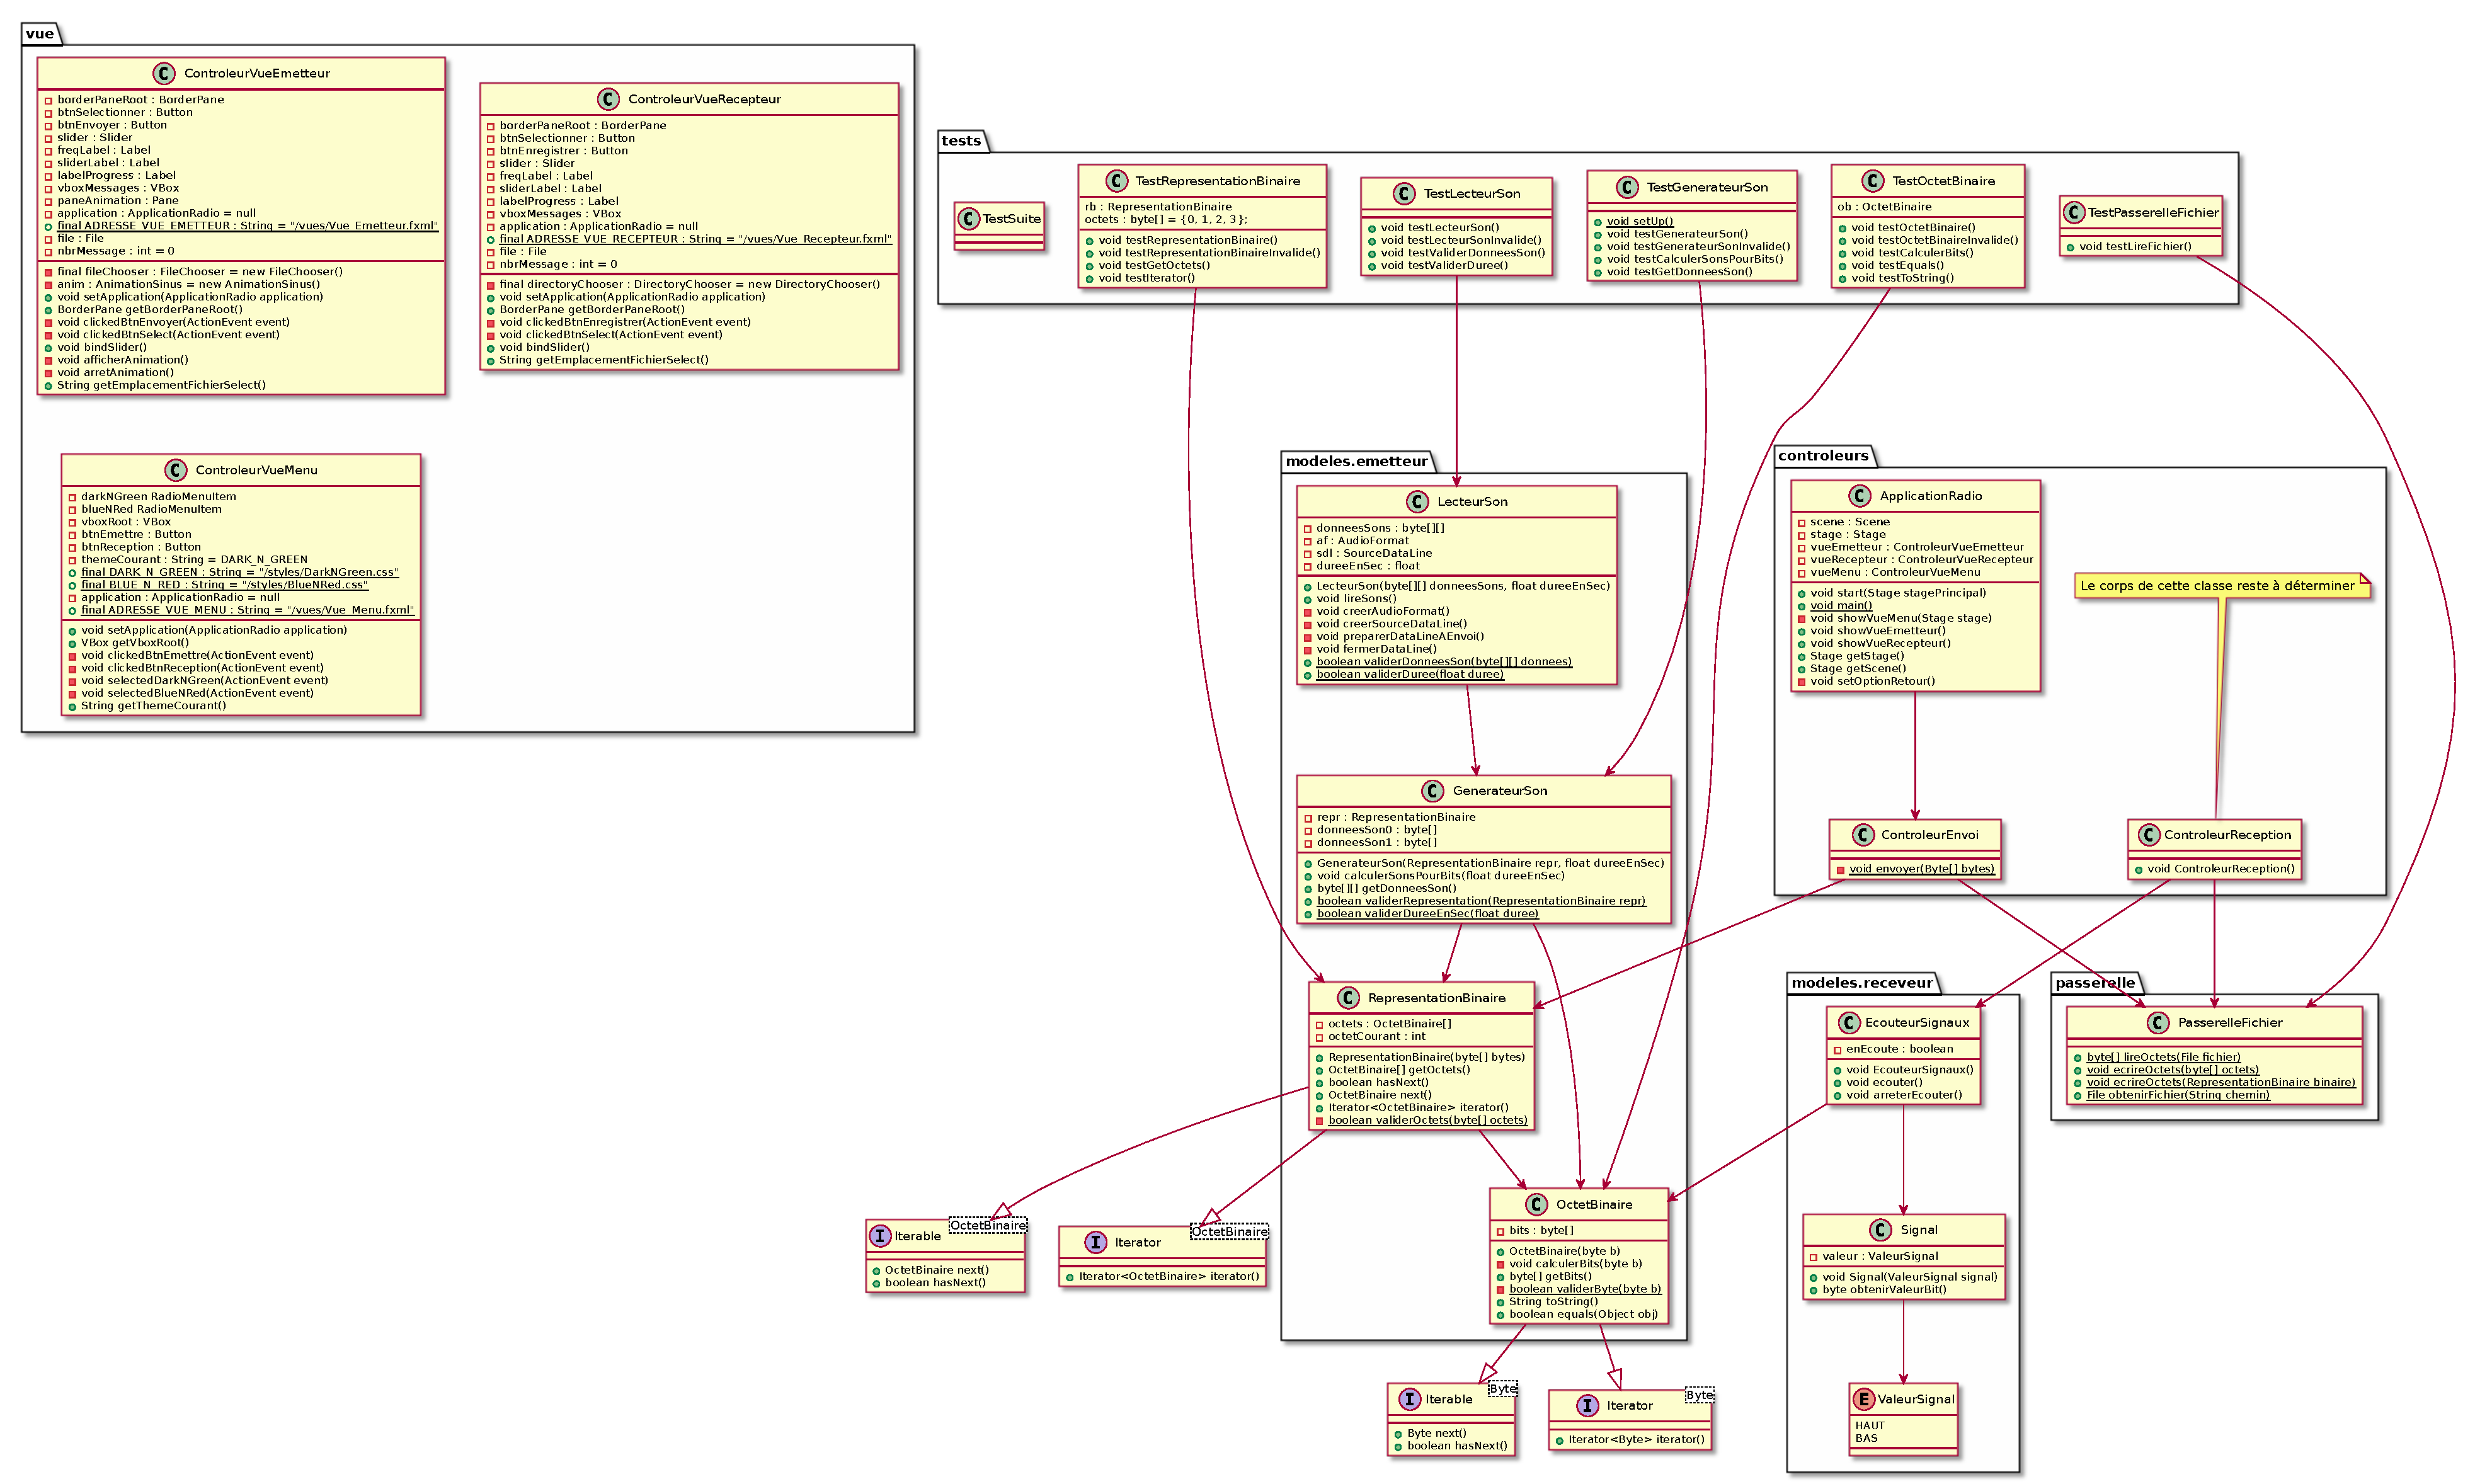
\includegraphics[width=0.8\linewidth]{images/diagramme_classes.pdf}
    \end{figure}

\section{Échéancier}
    \paragraph{Échéancier :}
Utilisation d'un échancier suivant le modèle du diagramme de Gantt réalisé à l'aide de MS Project. Il est divisé en trois captures d'écran à des fins pratiques.

\begin{figure}[ht!]
    \centering
    \caption{Échéancier partie 1}
    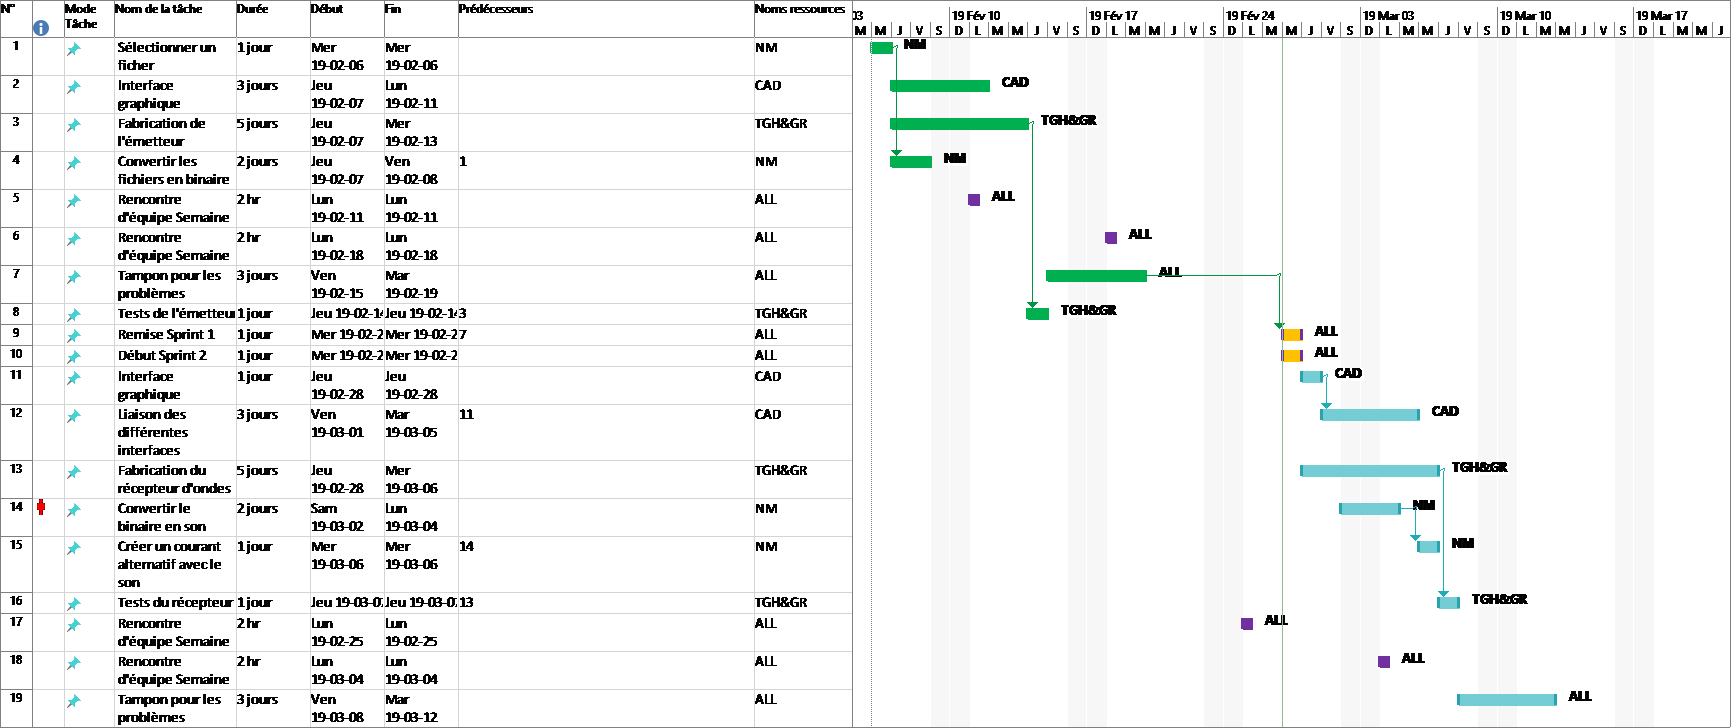
\includegraphics[width=0.8\linewidth]{images/echeancier/echeancier_Sprint_2_part1.png}
\end{figure}

\begin{figure}[ht!]
    \centering
    \caption{Échéancier partie 2}
    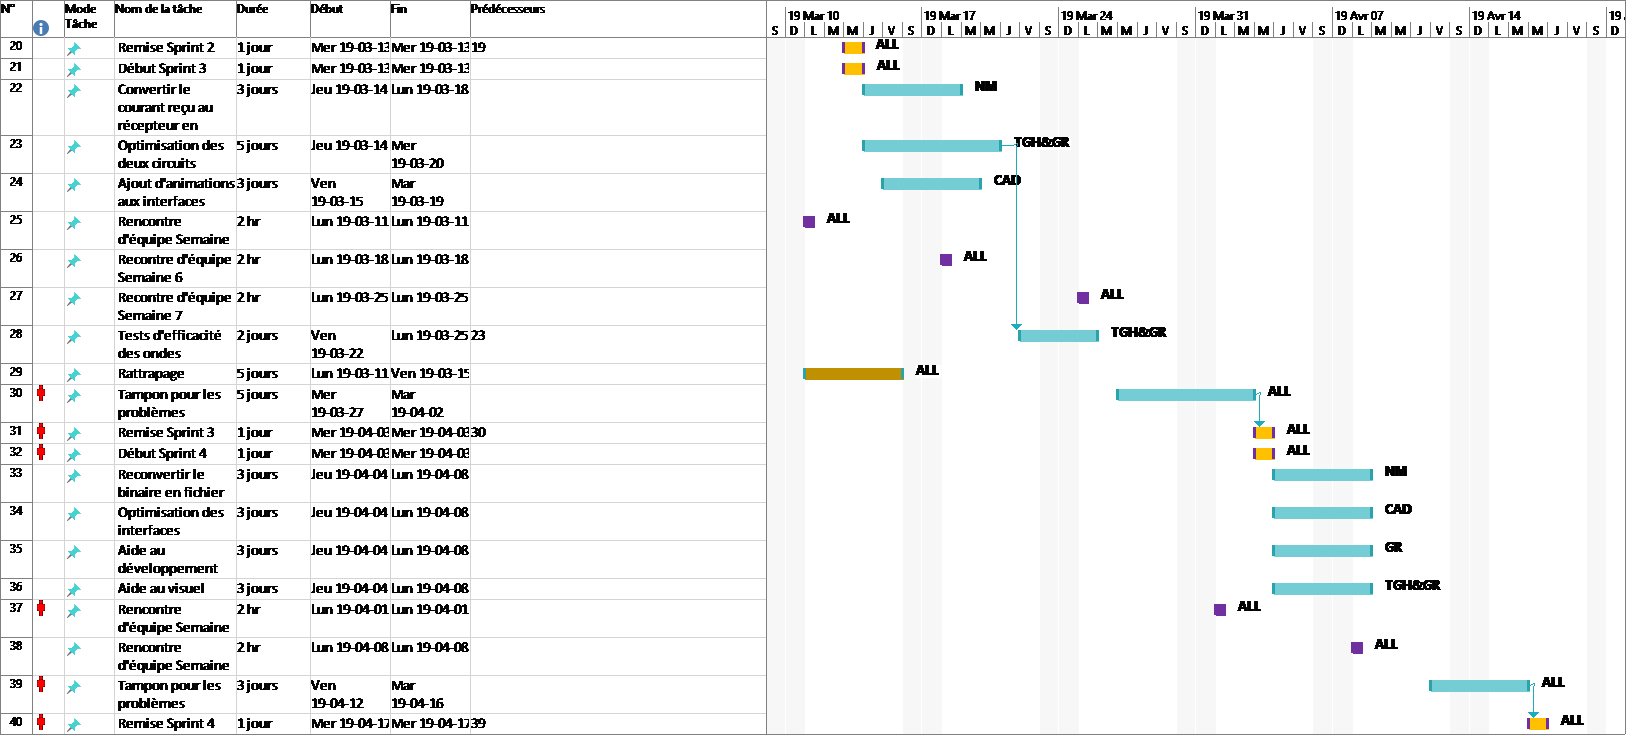
\includegraphics[width=0.8\linewidth]{images/echeancier/echeancier_Sprint_2_part2.png}
\end{figure}

\begin{figure}[ht!]
    \centering
    \caption{Échéancier partie 3}
    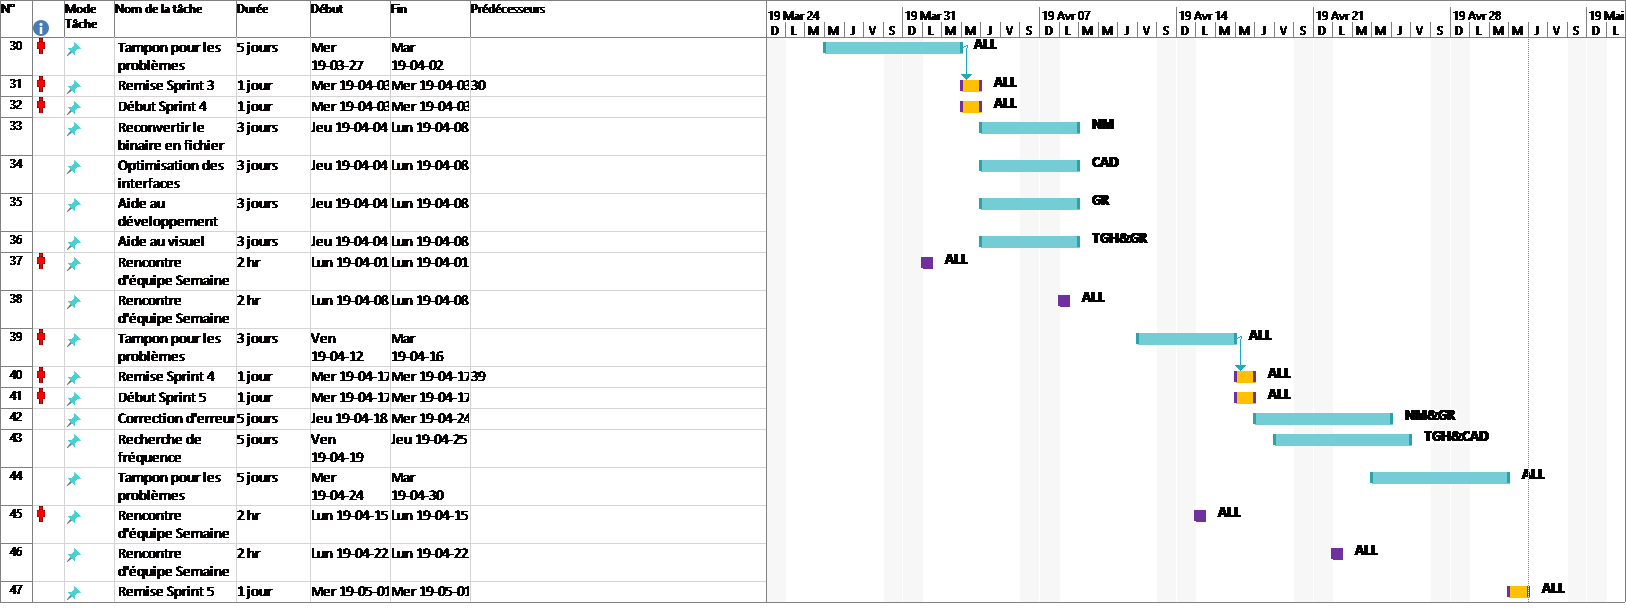
\includegraphics[width=0.8\linewidth]{images/echeancier/echeancier_Sprint_2_part3.png}
\end{figure}

\end{document}
